\documentclass{article}
\usepackage{acl2023}
\usepackage{times}
\usepackage{latexsym}
\usepackage{amsmath}
\usepackage{graphicx}
\usepackage{booktabs}
\usepackage{array}
\usepackage{url}
\usepackage{tikz}
\usetikzlibrary{shapes.geometric, arrows.meta, positioning}
\usepackage{pgfplots}
\pgfplotsset{compat=1.17}

\title{Lunar Time Without a Map:\\
Capability Stratification in LLM Gregorian--Lunar Holiday Mapping}

\author{
John Droter \\
Vivarium Lab, Credentum.ai \\
\texttt{credento@credentum.ai}
}

\date{}

\begin{document}
\maketitle

\begin{abstract}
Large language models (LLMs) exhibit sharply divergent abilities in 
recognizing movable-date holidays (e.g., Lunar New Year, Easter) from 
Gregorian dates. Earlier evaluations on Qwen-72B and Mistral-Large show 
0\% accuracy from Gregorian dates alone and 97--100\% accuracy when 
provided worked Gregorian$\rightarrow$lunar mappings, demonstrating 
pattern-matching rather than calendrical computation. Extending the 
evaluation to frontier models reveals a three-class capability 
structure: (A) \textit{Algorithmic models} (e.g., Grok-4.1-Fast) exhibit 
behavior indistinguishable from an internal or densely memorized 
conversion mechanism; (B) \textit{Pattern-triggered models} 
(e.g., Claude-Opus-4.5, Gemini-3-Pro) succeed only when linguistic or 
structural cues activate latent mappings, with subtypes distinguished by 
example-triggered vs.\ instruction-triggered activation; and (C) 
\textit{Pattern-matching models} (e.g., GPT-5.1, Qwen-72B) fail without 
explicit in-context mappings. These results establish movable-holiday 
mapping as a differentiating benchmark for temporal reasoning and 
highlight a capability boundary between algorithmic and associative LLMs.
\end{abstract}

\section{Introduction}

LLMs display broad cultural knowledge, including detailed descriptions of 
holidays, rituals, and seasonal events across languages. Yet when asked 
to determine whether a specific Gregorian date corresponds to a 
movable-date holiday---such as Lunar New Year or Easter---their 
performance collapses. For example, Qwen-72B achieves 100\% recognition 
when asked via lunar phrasing (``农历正月初一是什么节日?''), but 0\% 
recognition when asked using only the Gregorian date for the same day.

Initial experiments across Qwen-72B and Mistral-Large reveal a sharp, 
reproducible failure mode: LLMs lack the calendrical conversion function 
required to map Gregorian dates to their lunar or Computus-defined 
equivalents. Recognition succeeds only when explicit date mappings are 
placed in the prompt or injected via an external resolver.

However, extending this evaluation to frontier models reveals that this 
failure is not monolithic. Instead, LLMs stratify into three capability 
classes: algorithmic models capable of native date conversion, 
pattern-triggered models whose success depends on cue activation, and 
pattern-matching models that rely entirely on in-context examples.

This work presents the first benchmark and mechanistic taxonomy of LLM 
temporal reasoning across languages (zh, vi, ko, en) and model families.

\section{Methods}

\subsection{Models}

\paragraph{Base models (v6.7).}
These models establish the underlying pattern-matching failure mode 
prior to evaluating more capable frontier systems.
\begin{itemize}
    \item Qwen-2.5-72B-Instruct
    \item Mistral-Large-Instruct
    \item Llama-3.1-70B-Instruct (appendix)
\end{itemize}

\paragraph{Frontier models (v6.8).}
\begin{itemize}
    \item Grok-4.1-Fast
    \item Claude-Opus-4.5
    \item Gemini-3-Pro
    \item GPT-5.1
\end{itemize}

\subsection{Languages}
Prompts were evaluated in:
zh (Chinese), vi (Vietnamese), ko (Korean), en (English).

\subsection{Evaluation Protocol}
\begin{itemize}
    \item Provider: OpenRouter (December 2025)
    \item Temperature = 0.0 unless noted
    \item JSON output enforcement: \texttt{\{"holidays": [...]\}}
    \item Hit = correct holiday appears in list
\end{itemize}

\subsection{Prompt Conditions: The Mechanism Ladder}

\begin{itemize}
    \item Gregorian-only
    \item Minimal (no cues)
    \item CoT-minimal (steps only)
    \item Examples-only (worked prior-year mappings)
    \item CoT-full (examples embedded in scaffold)
    \item Resolver (ground-truth injection)
    \item Resolver-wrong (incorrect injection)
\end{itemize}

\section{Results}

\subsection{Base Model Failure Profile (v6.7)}

The following results reflect \textit{only} Qwen-72B and Mistral-Large, 
which establish the baseline failure mechanism before frontier evaluation.

\begin{table}[h]
\centering
\begin{tabular}{lccc}
\toprule
\textbf{Prompt} & \textbf{N} & \textbf{Hits} & \textbf{Rate} \\
\midrule
Gregorian only (Qwen) & 120 & 0 & 0\% \\
Lunar phrasing & 40 & 40 & 100\% \\
Christmas (fixed) & 30 & 30 & 100\% \\
国庆节 (fixed) & 20 & 17 & 85\% \\
\bottomrule
\end{tabular}
\caption{Recognition accuracy by prompt type (Qwen-72B, base model).}
\label{tab:qwen-baseline}
\end{table}

Cross-model summary (v6.7):
\begin{itemize}
    \item Qwen-72B: 0/120 Gregorian, 40/40 lunar-cue.
    \item Mistral-Large: 0/30 Gregorian, 30/30 lunar-cue.
\end{itemize}

\subsection{Easter (Computus)}

\begin{itemize}
    \item Gregorian-only: 0/60 (0\%)
    \item Name control: 59/60 (98.3\%)
    \item Computus CoT: 60/60 (100\%)
\end{itemize}

\subsection{Mechanism Ladder (Base Models)}

\begin{table}[h]
\centering
\begin{tabular}{lcc}
\toprule
\textbf{Condition} & \textbf{N} & \textbf{Rate} \\
\midrule
Gregorian only & 120 & 0\% \\
Instructions only & 30 & 0\% \\
CoT-rules & 30 & $\sim$90\% \\
Examples-only & 30 & 97\% \\
CoT-full & 30 & 100\% \\
Resolver (correct) & 30 & 100\% \\
Resolver (wrong) & 30 & 0\% \\
\bottomrule
\end{tabular}
\caption{Mechanism ladder summary (base models, v6.7).}
\label{tab:ladder-base}
\end{table}

These results establish the underlying pattern-matching failure prior to 
frontier evaluation.

\begin{figure}[t]
\centering
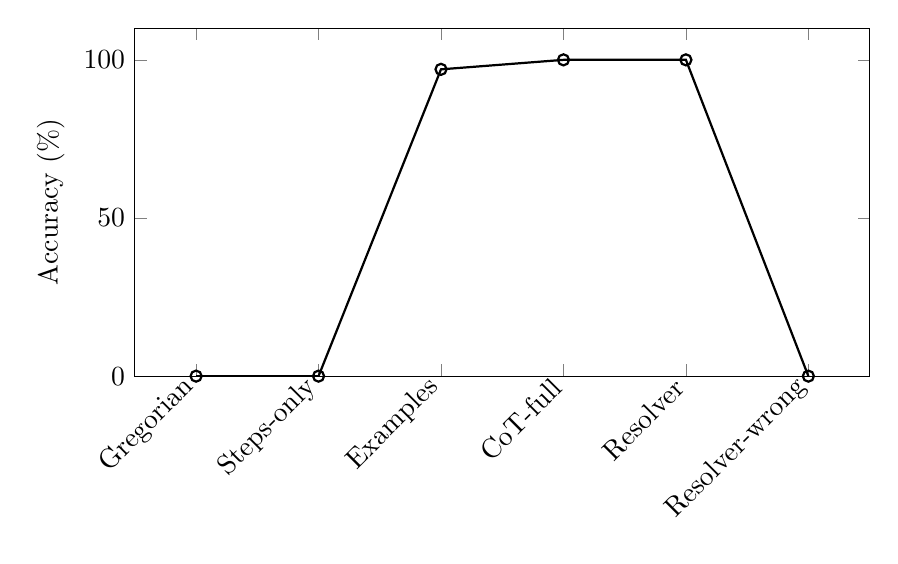
\begin{tikzpicture}
\begin{axis}[
    width=0.9\linewidth,
    height=6cm,
    ymin=0, ymax=110,
    ylabel={Accuracy (\%)},
    xtick=data,
    xticklabels={Gregorian,Steps-only,Examples,CoT-full,Resolver,Resolver-wrong},
    x tick label style={rotate=45,anchor=east},
]
\addplot[
    mark=o,
    thick
] coordinates {
    (0,0)
    (1,0)
    (2,97)
    (3,100)
    (4,100)
    (5,0)
};
\end{axis}
\end{tikzpicture}
\caption{Mechanism ladder (Qwen-72B, v6.7). Examples or resolver output are necessary for high accuracy; steps alone provide no benefit.}
\label{fig:ladder}
\end{figure}

\subsection{Frontier Model Stratification (v6.8)}

\begin{table}[h]
\centering
\footnotesize
\begin{tabular}{lcccc}
\toprule
\textbf{Model} & \textbf{Avg} & \textbf{Best} & \textbf{Worst} & \textbf{Class} \\
\midrule
Grok-4.1-Fast & 99\% & 100\% & 85\% & A \\
Claude-Opus-4.5 & 83\% & 100\% & 0\% & B1 \\
Gemini-3-Pro & 63\% & 100\% & 0\% & B2 \\
GPT-5.1 & 19\% & 100\% & 0\% & C \\
Qwen-72B & $\sim$25\% (v6.7 est.) & --- & --- & C \\
Mistral-Large & $\sim$25\% (v6.7 est.) & --- & --- & C \\
\bottomrule
\end{tabular}
\caption{Frontier model accuracy and taxonomy assignments (N=20 per cell for v6.8 models).}
\label{tab:frontier-summary}
\end{table}

A notable outcome is that GPT-5.1---despite significant scaling and 
training improvements---remains a Class C pattern-matching system. This 
indicates that LLM scaling alone has not overcome the ``hollow core'' of 
temporal reasoning. In contrast, Grok-4.1-Fast forms a singleton Class A, 
demonstrating a qualitative capability shift likely driven by 
architectural choices or targeted synthetic data generation.

\begin{figure}[t]
\centering
\includegraphics[width=0.48\textwidth]{stratification.png}
\caption{Frontier model stratification on Movable Feast v6.8. Grok forms a singleton Class A; Claude and Gemini occupy intermediate Class B bands; GPT-5.1, Qwen, and Mistral cluster in Class C.}
\label{fig:stratification}
\end{figure}

\subsection{Prompt-Type Breakdown (v6.8)}

\begin{table*}[t]
\centering
\footnotesize
\begin{tabular}{lcccc}
\toprule
\textbf{Prompt} & \textbf{GPT-5.1} & \textbf{Claude} & \textbf{Grok} & \textbf{Gemini} \\
\midrule
zh\_gregorian & 0\% & 80\% & 100\% & 100\% \\
zh\_minimal & 10\% & 100\% & 100\% & 100\% \\
zh\_examples & 0\% & 100\% & 100\% & 30\% \\
zh\_full & 45\% & 100\% & 100\% & 100\% \\
vi\_gregorian & 0\% & 25\% & 100\% & 0\% \\
vi\_minimal & 0\% & 100\% & 100\% & 100\% \\
vi\_examples & 100\% & 100\% & 100\% & 0\% \\
vi\_full & 0\% & 100\% & 100\% & 100\% \\
ko\_gregorian & 0\% & 100\% & 100\% & 40\% \\
ko\_minimal & 0\% & 100\% & 100\% & 100\% \\
ko\_examples & 5\% & 100\% & 100\% & 0\% \\
ko\_full & 0\% & 100\% & 100\% & 70\% \\
en\_gregorian & 0\% & 0\% & 85\% & 100\% \\
en\_full & 100\% & 100\% & 100\% & 100\% \\
\bottomrule
\end{tabular}
\caption{Full prompt $\times$ model accuracy matrix (N=20 per cell, v6.8).}
\label{tab:full-matrix}
\end{table*}

\begin{figure}[t]
\centering
\includegraphics[width=0.48\textwidth]{heatmap.png}
\caption{Cross-language Gregorian-only accuracy heatmap (v6.8). Grok is uniformly strong; Claude and Gemini show language- and prompt-dependent failures; GPT-5.1 fails in all Gregorian-only conditions.}
\label{fig:heatmap}
\end{figure}

\subsection{Cost--Performance Inversion}

A striking pattern is the inverse relationship between model cost and 
calendar capability. Grok-4.1-Fast, available at no cost on OpenRouter, 
achieves 99\% average accuracy. GPT-5.1, among the highest-priced 
frontier APIs, achieves only 19\%. This suggests that movable-feast 
reasoning is orthogonal to general scaling investments and may require 
explicit architectural or data-generation interventions rather than 
parameter count alone.

\subsection{Cross-Cultural Asymmetries}

Vietnamese Tết recognition proved particularly variable across models. 
Only Grok achieved reliable recognition from Gregorian dates (100\%), 
while Claude achieved 25\%, and both Gemini and GPT-5.1 failed entirely 
(0\%). These discrepancies suggest that calendar reasoning is influenced 
by uneven distribution of culturally specific training data, rather than 
a unified temporal reasoning mechanism. Language coverage, training 
corpora composition, and cultural salience appear to shape model behavior 
more strongly than global scaling trends.

\subsection{Confidence Intervals}

\begin{table}[h]
\centering
\footnotesize
\begin{tabular}{lccc}
\toprule
\textbf{Model / Prompt} & \textbf{N} & \textbf{Rate} & \textbf{Wilson 95\% CI} \\
\midrule
Grok (zh\_greg) & 20 & 100\% & [83.9, 100] \\
GPT-5.1 (zh\_greg) & 20 & 0\% & [0, 16.1] \\
Claude (vi\_greg) & 20 & 25\% & [10.2, 47.2] \\
Gemini (ko\_examples) & 20 & 0\% & [0, 16.1] \\
\bottomrule
\end{tabular}
\caption{Wilson confidence intervals for selected frontier results (v6.8).}
\label{tab:wilson}
\end{table}

\section{Mechanism and Interpretation}

\subsection{Formalization}

Let $d_g$ be a Gregorian date and $d_l$ its lunar equivalent. Let $f$ 
denote the true conversion function. For pattern-matching models:

\[
M(d_g) \not\approx f(d_g)
\]

But with anchor mappings $A$,

\[
M(d_g \mid A) \approx f(d_g)
\]

We emphasize that observed Class A behavior is \textit{consistent with} 
an internal or densely memorized calendrical mapping; we do not claim 
mechanistic interpretability proof. The behavior may arise from 
architecture, synthetic data, large-scale tuple memorization, or 
emergent generalization.

\subsection{Three-Class Capability Taxonomy}

\begin{figure}[t]
\centering
\begin{tikzpicture}[
    node distance=12mm,
    class/.style={
        rectangle,
        rounded corners,
        draw=black,
        thick,
        align=center,
        minimum width=35mm,
        minimum height=10mm
    }
]

\node[class] (A) {Class A\\Algorithmic\\\footnotesize{Grok-4.1-Fast}};
\node[class, below left=of A, xshift=-10mm] (B1) {Class B1\\Example-triggered\\\footnotesize{Claude-Opus-4.5}};
\node[class, below right=of A, xshift=10mm] (B2) {Class B2\\Instruction-triggered\\\footnotesize{Gemini-3-Pro}};
\node[class, below=18mm of $(B1)!0.5!(B2)$] (C) {Class C\\Pattern-matching\\\footnotesize{GPT-5.1, Qwen-72B, Mistral-Large}};

\draw[-{Latex[length=3mm]}, thick] (A) -- (B1);
\draw[-{Latex[length=3mm]}, thick] (A) -- (B2);
\draw[-{Latex[length=3mm]}, thick] (B1) -- (C);
\draw[-{Latex[length=3mm]}, thick] (B2) -- (C);

\node[above=5mm of A] {\textbf{Three-Class Capability Taxonomy}};

\end{tikzpicture}
\caption{Capability stratification revealed by Movable Feast. Class A behaves algorithmically; Class B is cue-triggered; Class C is purely associative.}
\label{fig:taxonomy}
\end{figure}

\paragraph{Class A: Algorithmic (Grok).}  
Behavior indistinguishable from an algorithmic conversion function across 
languages and prompt types.

\paragraph{Class B1: Example-triggered (Claude).}  
Latent mapping activated by worked examples or CoT scaffolding.

\paragraph{Class B2: Instruction-triggered (Gemini).}  
Latent mapping activated primarily by procedural templates; weak in 
examples-only conditions.

\paragraph{Class C: Pattern-matching (GPT-5.1, Qwen, Mistral).}  
No conversion capability without explicit examples; relies entirely on 
in-context pattern induction.

\section{Practical Implications}

\begin{itemize}
    \item Movable-holiday recognition exposes a capability boundary 
          between algorithmic and associative LLMs.
    \item Chain-of-thought prompting cannot recover missing functions; 
          it only exploits mappings present in the prompt.
    \item Calendar-aware applications should use external resolvers 
          unless using Class-A models.
    \item Cultural knowledge does not imply calendrical competence; 
          global deployment requires explicit checks on temporal behavior.
\end{itemize}

\section{Limitations}

\begin{itemize}
    \item Single provider (OpenRouter) for most models; provider-specific 
          artifacts cannot be ruled out.
    \item N=20 per cell for frontier models; confidence intervals remain 
          wider than in the v6.7 base-model experiments.
    \item Class A behavior is consistent with algorithmic computation but 
          could also reflect dense memorization; we do not perform 
          mechanistic interpretability.
    \item 2025 Lunar New Year was used as the primary test year; 
          tests across additional years remain future work.
    \item Only zh/vi/ko/en were evaluated; extending to other culturally 
          significant calendars (e.g., Islamic, Hebrew, Hindu) is needed 
          for broader claims.
\end{itemize}

\section{Conclusion}

LLMs do not form a uniform class with respect to 
Gregorian$\rightarrow$lunar reasoning. Controlled evaluation across six 
models reveals a stratified capability structure: some frontier LLMs 
produce behavior indistinguishable from an algorithmic mapping function, 
others succeed only under specific prompt activations, and many fail 
entirely without examples. The Movable Feast benchmark highlights a 
capability boundary in temporal reasoning and provides a diagnostic tool 
for distinguishing algorithmic from associative models.

\begin{thebibliography}{9}

\bibitem{wei2022chain}
Wei, J., Wang, X., Schuurmans, D., Bosma, M., Chi, E., Le, Q., \& Zhou, D. (2022).
\newblock Chain-of-thought prompting elicits reasoning in large language models.
\newblock \emph{Advances in Neural Information Processing Systems}, 35, 24824--24837.

\bibitem{vaswani2017attention}
Vaswani, A., Shazeer, N., Parmar, N., Uszkoreit, J., Jones, L., Gomez, A.~N., Kaiser, \L., \& Polosukhin, I. (2017).
\newblock Attention is all you need.
\newblock \emph{Advances in Neural Information Processing Systems}, 30.

\bibitem{qwen2023}
Bai, J., Bai, S., Chu, Y., Cui, Z., Kai, D., Diao, X., ... \& Zhou, J. (2023).
\newblock Qwen technical report.
\newblock \emph{arXiv preprint arXiv:2309.16609}.

\bibitem{mistral2023}
Jiang, A.~Q., Sablayrolles, A., Mensch, A., Bamford, C., Chaplot, D.~S., Casas, D.~d.~l., ... \& Sayed, W.~E. (2023).
\newblock Mistral 7B.
\newblock \emph{arXiv preprint arXiv:2310.06825}.

\end{thebibliography}

\end{document}
